\documentclass{standalone}
\usepackage{tikz}

\begin{document}
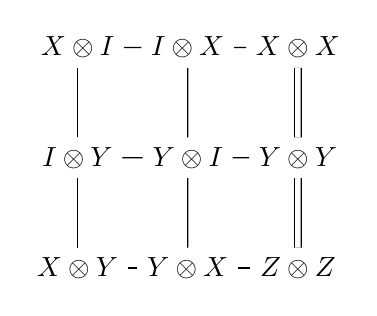
\begin{tikzpicture}[scale=1.4, 
% every node/.style={scale=0.9}
]
\node (XY) at (0,0) {$X \otimes Y$};
\node (YX) at (1,0) {$Y \otimes X$};
\node (ZZ) at (2,0) {$Z \otimes Z$};
\node (IY) at (0,1) {$I \otimes Y$};
\node (YI) at (1,1) {$Y \otimes I$};
\node (YY) at (2,1) {$Y \otimes Y$};
\node (XI) at (0,2) {$X \otimes I$};
\node (IX) at (1,2) {$I \otimes X$};
\node (XX) at (2,2) {$X \otimes X$};
\draw (XY) -- (IY) -- (XI) ;
\draw (YX) -- (YI) -- (IX) ;
\draw [double distance = 2pt] (ZZ) -- (YY) -- (XX) ;
\draw (XY) -- (YX) -- (ZZ) ;
\draw (IY) -- (YI) -- (YY) ;
\draw (XI) -- (IX) -- (XX) ;
\end{tikzpicture}
\end{document}